\section{Optimierung der Parameter des BDT-Algorithmus}
\label{sec:bdt_optimization}
Bei der BDT-Methode wurde je nach Parameter-Konstellation der AMS schlechter wenn nicht der volle Eingabevariablensatz verwendet wurde. Daher wurde der volle Satz an Variablen verwendet. Um die optimalen Parameter für den BDT zu finden, haben wir für die Parameter
\begin{itemize}
	\item NTrees
	\item NEventsMin
	\item Shrinkage
	\item nCuts
	\item MaxDepth
\end{itemize} 
sinnvolle Bereiche festgelegt und suchten in diesem Parameterraum den besten AMS. Da die Laufzeit des Trainings für jeden Punkt im Parameterraum in der Größenordnung von Minuten liegt und wir 5 Parameter haben, lassen sich herkömmliche Optimierungsalgorithmen nicht sinnvoll anwenden.\\
Um einen Überblick zu erhalten ob es gewisse Bereiche im Parameterraum gibt, in denen der AMS generell besser ist, haben wir 1389 mal zufällige Parameter gewählt und den AMS dazu gespeichert. Wenn ein neuer Bestwert erreicht wurde, wurden die kontinuierlichen Parameter NEventsMin und Shrinkage gaußverteilt um die zugehörigen Werte erzeugt.\\
Wie in den Abbildungen \ref{AMS-distribution-plots} (a)-(e) zu erkennen ist, gibt es für einzelne Parameter keinen optimalen Wert. Die Auswirkungen der Parameter sind korreliert und eine Optimierung in nur einem Parameter nicht möglich. Des besten AMS erreichten wir mit
\begin{itemize}
	\item NTrees = 167
	\item NEventsMin = 7.28244760204
	\item Shrinkage = 0.0530833026321
	\item nCuts = 275
	\item MaxDepth  = 9  ,
\end{itemize} 
was auf den Trainingsdaten zu einem AMS-Wert von $0{,}773$ führte.

\begin{figure}[!t]
  \begin{tabular}[b]{cc}
	  \begin{subfigure}[b]{0.5\linewidth}
	   	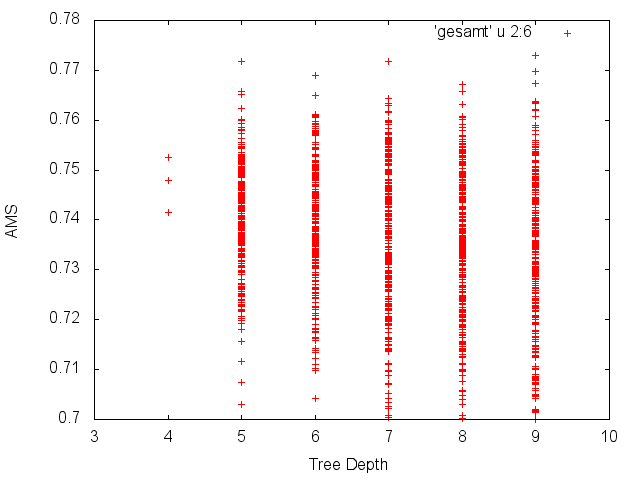
\includegraphics[width=\linewidth]{sections/parameter_optimization_bdt/Depth.png}
 		\caption[]{}
		\label{fig:bdt_Depth}
  	  \end{subfigure} &
  	  \begin{subfigure}[b]{0.5\linewidth}
  	  	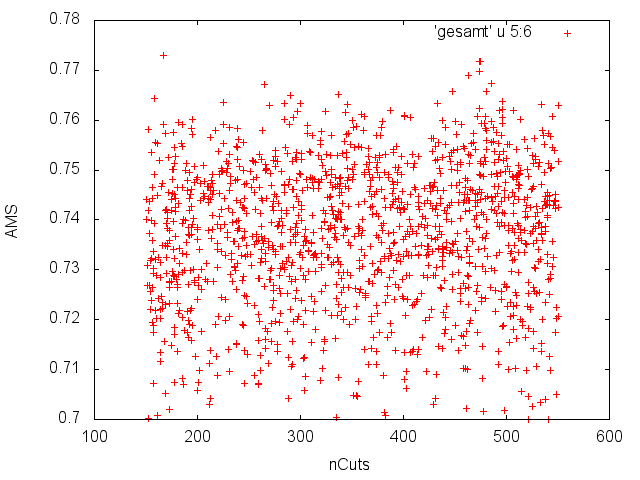
\includegraphics[width=\linewidth]{sections/parameter_optimization_bdt/nCuts.png}
 		\caption[]{}
		\label{fig:bdt_nCuts}
  	  \end{subfigure} \\
  	  
  	  \begin{subfigure}[b]{0.5\linewidth}
	   	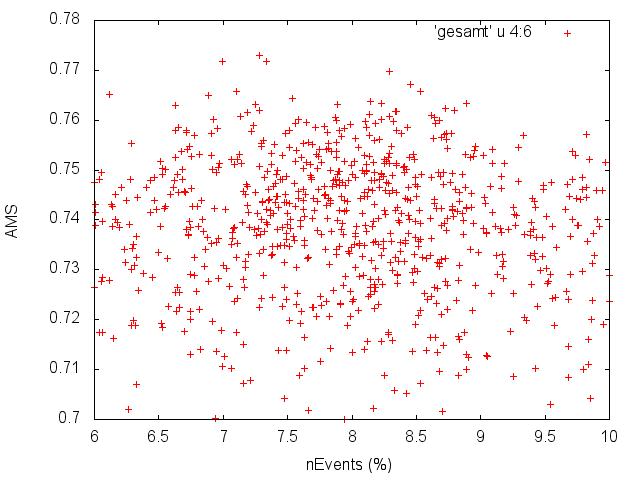
\includegraphics[width=\linewidth]{sections/parameter_optimization_bdt/nEvents.png}
 		\caption[]{}
		\label{fig:bdt_nEvents}
  	  \end{subfigure} &
  	  \begin{subfigure}[b]{0.5\linewidth}
  	  	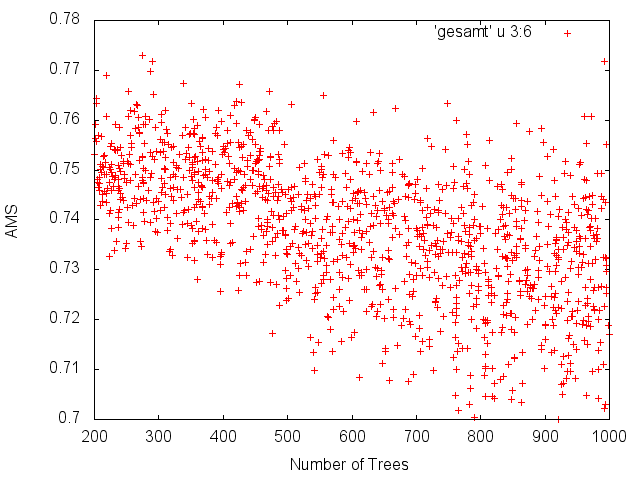
\includegraphics[width=\linewidth]{sections/parameter_optimization_bdt/Nt.png}
 		\caption[]{}
		\label{fig:bdt_Nt}
  	  \end{subfigure} \\
  	  
  	  \begin{subfigure}[b]{0.5\linewidth}
	   	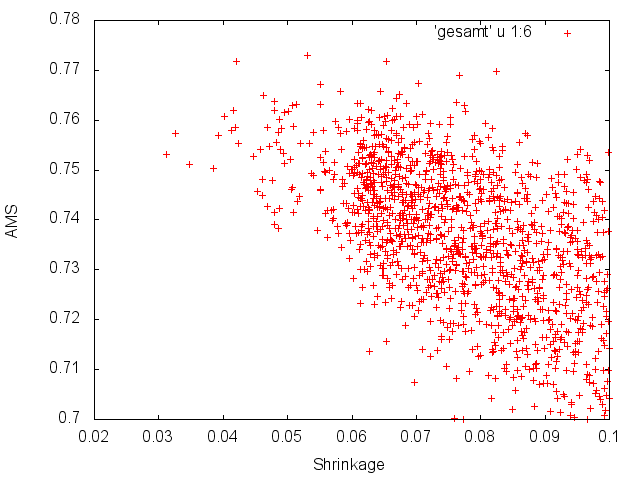
\includegraphics[width=\linewidth]{sections/parameter_optimization_bdt/Shrinkage.png}
 		\caption[]{}
		\label{fig:bdt_Shrinkage}
  	  \end{subfigure} &
  \end{tabular}
  \caption[AMS-Werte für die Parameter der Boosted Decision Trees]{AMS-Werte für die Parameter der Boosted Decision Trees als Scatter-Plots. Jeder Punkt entspricht einem Training.}
  \label{fig:AMS-distribution-plots}
\end{figure}